\subsection{Функция источника}
Спектр рентгеновской трубки является характеристическим, спектральная часть
 которого достаточно хорошо описывается двумя функциями Лоренца взятыми с
 весовыми коэффициентами (\ref{eq:source_spectral}).

 \begin{equation} \label{eq:source_spectral}
   g_{\lambda} (\lambda) = \frac{2\pi}{3}  \left \{ \frac{\delta\lambda_1}{(\lambda - \lambda_1)^2+
   (\delta \lambda_1)^2} + \frac{1}{2} \frac{\delta\lambda_2}{(\lambda-\lambda_1)^2+(\delta\lambda_1)^2} \right \}
  \end{equation}

  Плотность распределения количества потока электромагнитного излучения в зависимости от угла
  отстройки относительно прямолинейного распределения задается функцией Гаусса \ref{eq:source_angle}.

  \begin{equation} \label{eq:source_angle}
    g_{\vartheta} (\vartheta) = \frac{1}{\sigma \sqrt{ 2\pi}} exp  ( -\frac{\vartheta^2}{2\sigma^2} )
   \end{equation}
где $\sigma$ - параметр, который характеризует ширину углового распределения на половине высоты.

\begin{figure}[H]
  \centering
  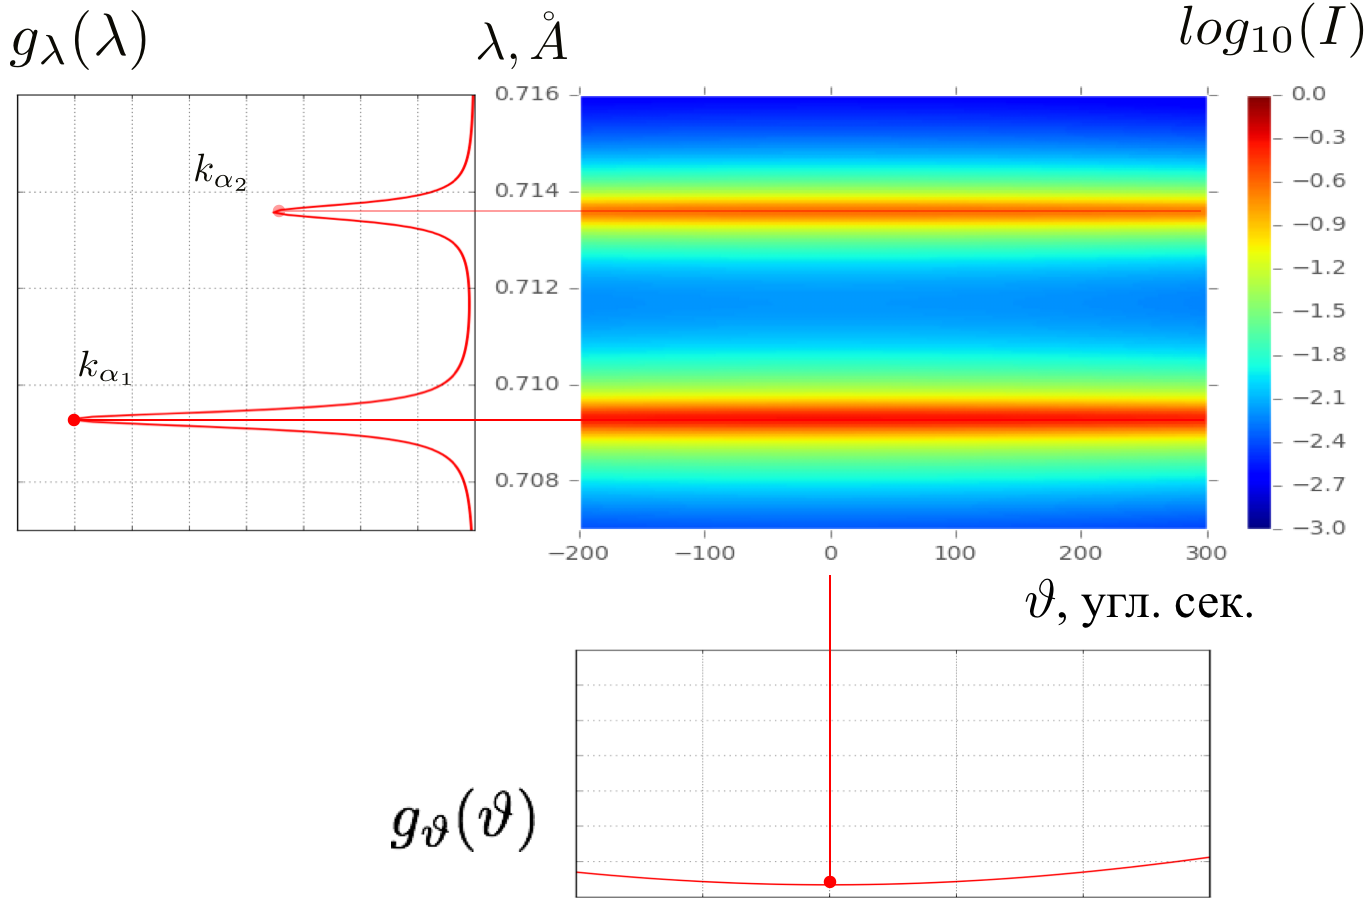
\includegraphics[width=0.6\textwidth]{images/source_distrubition.png}
  \caption{Спектрально – угловое распределение лабораторного источника рентгеновского
   излучения с молибденовым анодом, угловая полуширина распределения составляет $\sigma = 600$ угл. сек. }
  \label{ris:source_distrubition}
\end{figure}


 \subsection{Функция щелевых коллиматоров}
 \label{sec:slits_section}
 Рассмотрим преобразование пучка рентгеновского излучения проходящего через систему щелевых коллиматоров.
 \begin{figure}[H]
   \centering
   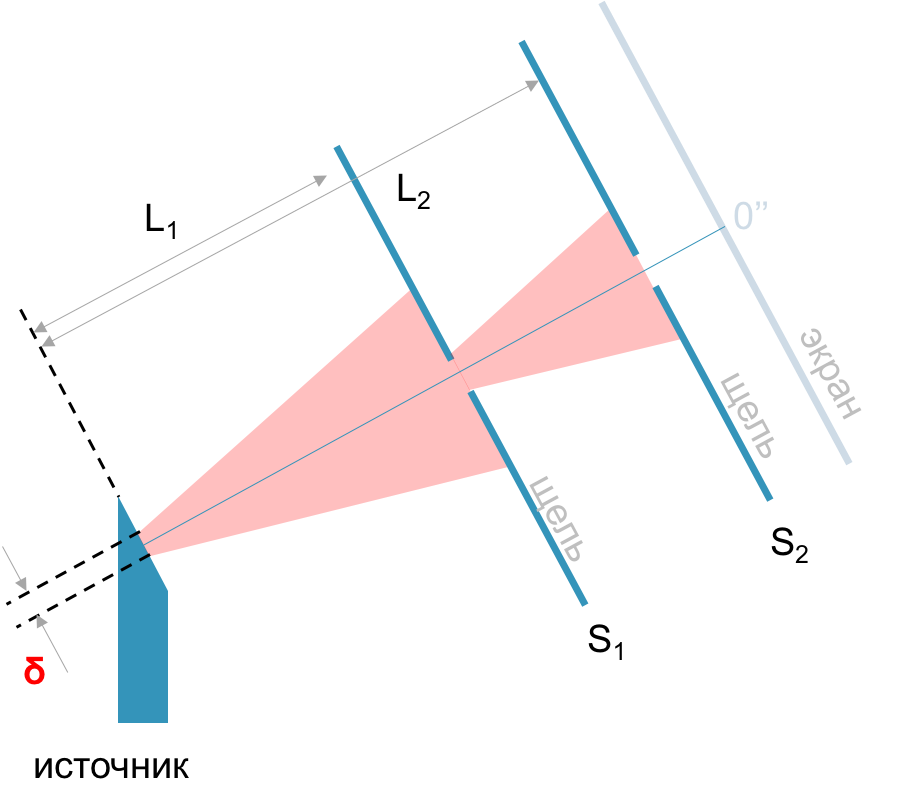
\includegraphics[width=0.6\textwidth]{images/for_slits.png}
   \caption{Схематичное представление щелевых устройств}
   \label{ris:for_slits}
 \end{figure}

На начальном этапе мы рассматривали модель точечного источника излучения $\delta = 0$.
В таком случае, интенсивность проходящего излучения будет определятся
одним щелевым устройством, которое является более узким в пересчете в угловые
координаты. Например, для фиксированных расстояний между элементами,
($L_1 = 570$ мм, $L_2 = 1005$ мм), в случае одинаковых линейных размеров щелей и точечного
источника, интенсивность будет определяться более удаленным щелевым устройством и
распределение интенсивности принимает вид ступеньки (рисунок ~\ref{ris:sourc_map_a}). Если источник является
 продолжительным $\delta \neq 0$, то угловое распределение интенсивности принимает более сложный вид, как показано на рисунке ~\ref{ris:sourc_map_b}.



 \begin{figure}[H]
   \centering
   \subfloat[Точечный источник]{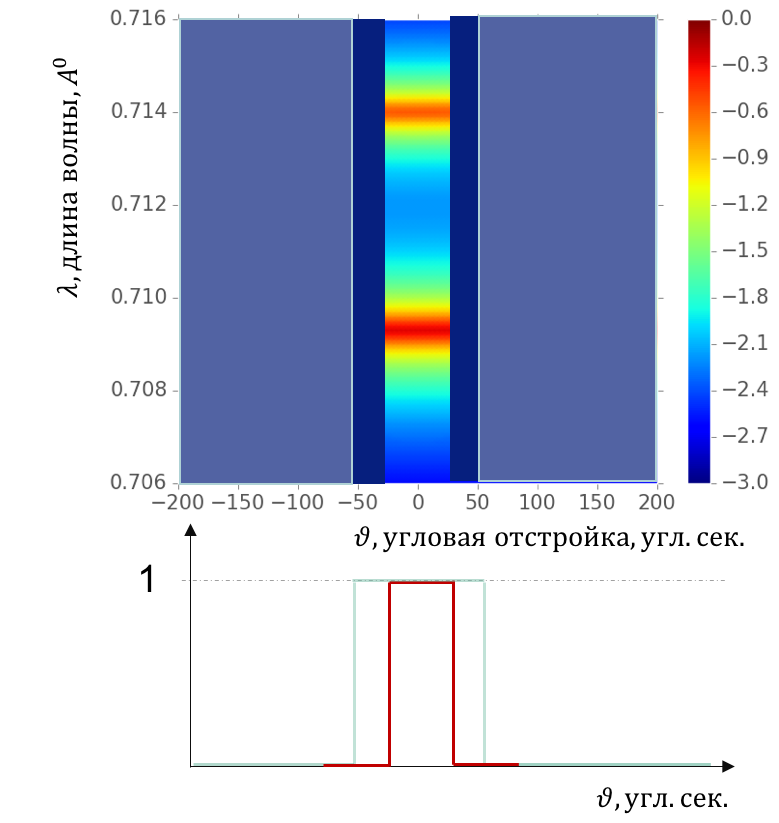
\includegraphics[width=0.5\textwidth]{images/point_sourc_map.png}\label{ris:sourc_map_a}}
   \hfill
   \subfloat[Источник с линейным размером $\delta = 0.2$ мм]{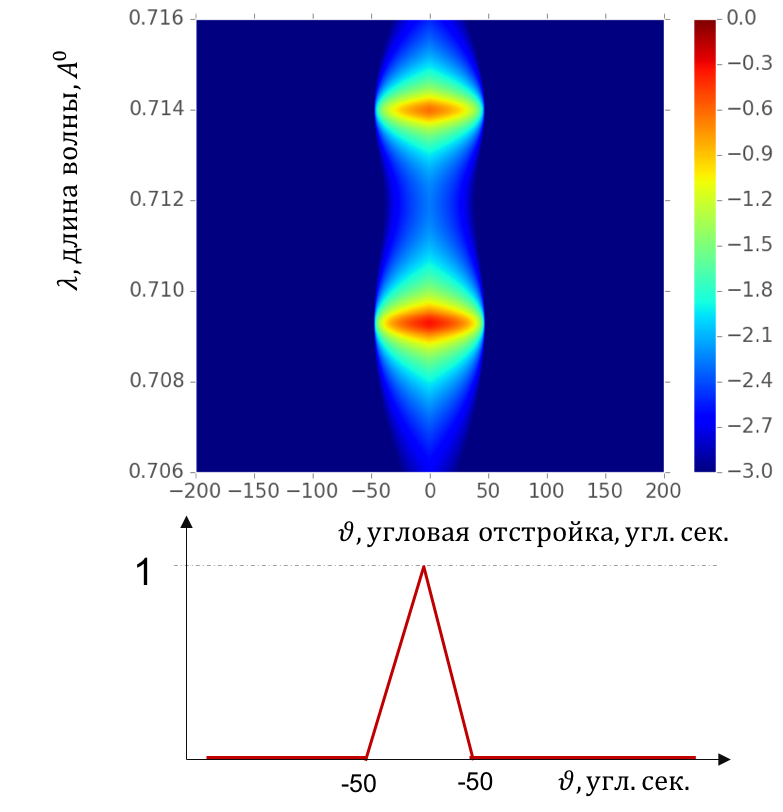
\includegraphics[width=0.5\textwidth]{images/wide_sourc_map.png}\label{ris:sourc_map_b}}
   \caption{Спектрально угловое распределение источника в система двух щелей}
   \label{ris:sourc_map}
 \end{figure}

 Необходимо отметить, что для описания дифракционного эксперимента важно расчитывать именно
 угловое распределение, т.е. знать количество и величину энергии квантов падающих под тем
 или иным углом на кристалл. Для того, чтобы это сделать нам необходимо посчитать площадь параллелограммов
 (рисунок \ref{ris:how_many_quants_use_parallelogr}),

 \begin{figure}[H]
   \centering
   \subfloat[Пропускная способность системы пропорциональна площади
   соответствующего параллелограмма ]{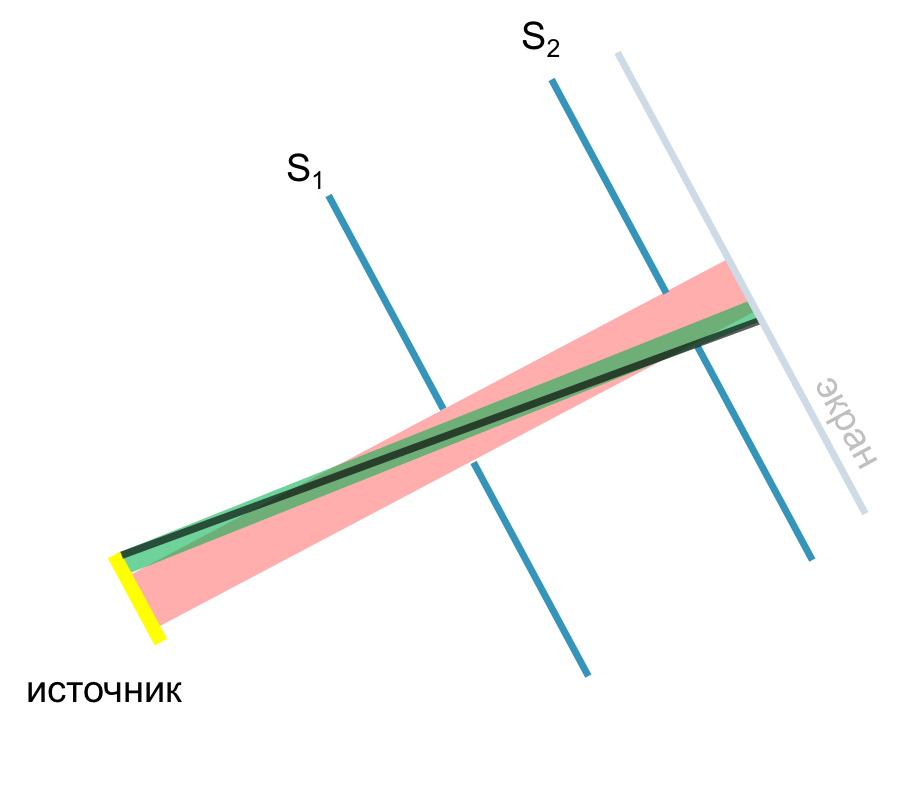
\includegraphics[width=0.45\textwidth]{images/how_many_quants_use_parallelogr_1.png}}
   \hfill
   \subfloat[Интенсивность на экране $\delta = 0.2$ мм,  \textcolor{mygreen}{Ось ординат $g_S(\vartheta)$}]{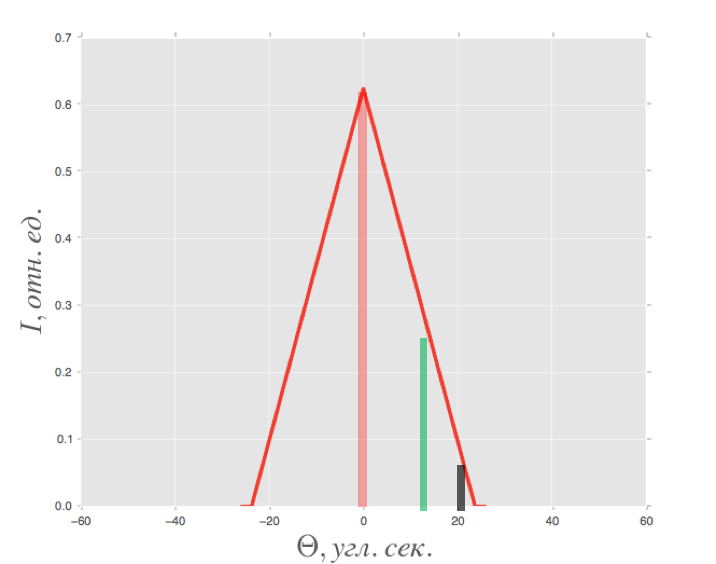
\includegraphics[width=0.45\textwidth]{images/how_many_quants_use_parallelogr_2.png}}
   \caption{Схематичное представление расчета интенсивности углового
   распределения излучения после прохождения системы щелевых коллиматоров}
   \label{ris:how_many_quants_use_parallelogr}
 \end{figure}
Более подробный расчет  $g_S(\vartheta)$ представлен в (\ref{sec:calc_slits_ability}).
На рисунке (\ref{ris:calc_slits_ability_res}) представлены результаты расчета пропускной способности системы двух щелей для некоторых параметров в
приближении точечного и продолжительного источника.

\begin{figure}[H]
  \centering
  \subfloat[$S_1 = S_2 = 50$ мкм; $\delta = 0.2$ мм;]{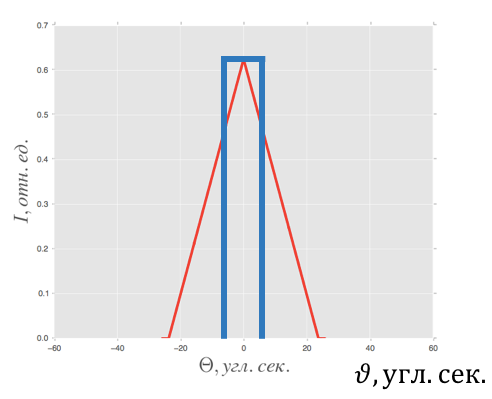
\includegraphics[height=6em]{images/calc_slits_ability_res_1.png}}
  \hfill
  \subfloat[$S_1 = 20$ мкм; $S_2 = 40$ мкм; $\delta = 0.2$ мм;]{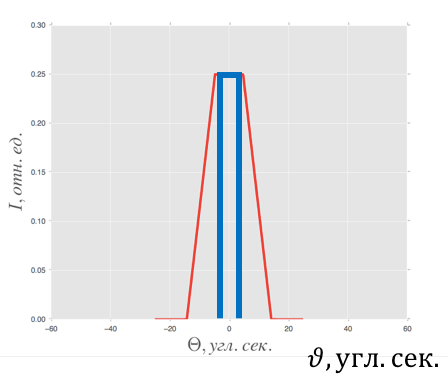
\includegraphics[height=6em]{images/calc_slits_ability_res_2.png}}
  \hfill
  \subfloat[$S_1 = 200$ мкм; $S_2 = 400$ мкм; $\delta = 0.2$ мм;]{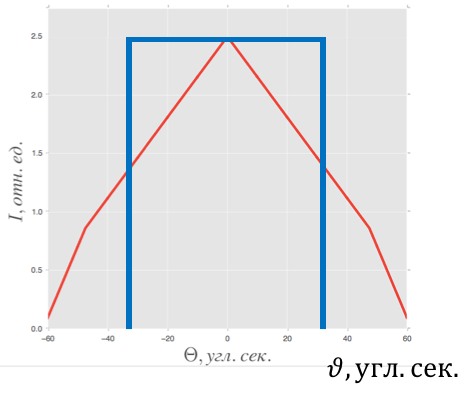
\includegraphics[height=6em]{images/calc_slits_ability_res_3.png}}
  \hfill
  \subfloat[$S_1 = 200$ мкм; $S_2 = 400$ мкм; $\delta = 0.1$ мм;]{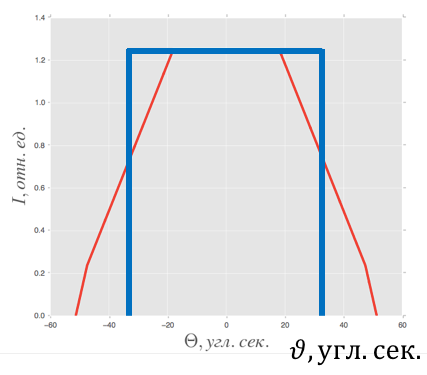
\includegraphics[height=6em]{images/calc_slits_ability_res_4.png}}
  \caption{$L_1 = 570$ мм; $L_2 = 1005 $ мм \textcolor{mygreen}{ Ось ординат $g_S(\vartheta)$}}
  \label{ris:calc_slits_ability_res}
\end{figure}

Анализ показывает что перегиб (рисунок \ref{ris:calc_slits_ability_res}) возникает вследствие переходного
процесса от точечного источника к бесконечному, т.е. на меньших углах плотность излучения определяется ближайшей
щелью к источнику, а после некоторого угла определяющей становится более удаленная \textcolor{mygreen}{НАРИСОВАТЬ РИСУНОК}(рисунок ).

\subsubsection{Отражение от одного кристалла}
  Постепенно будем наполнять схему и внесем один идеальный кристаллический элемент.
  Кристалл регламентируется уже не только угловой составляющей пучка, но и берет в учет энергию.

  Спектрально-угловое распределение после отражающего кристаллического элемента задается выражением
  \begin{equation} \label{eq:monochromator_spectra}
    P(\vartheta,\lambda) = g_{\lambda}(\lambda)g_{\vartheta}(\vartheta) P(\vartheta - \frac{\lambda - \lambda_1}{\lambda_1}\tan(\theta_B))
   \end{equation}
где $P$ - соответствует (\ref{eq:KDO_self}), $\lambda_1$ - длина волны излучения от которой ведется отсчет углов $\vartheta$.
\begin{figure}[H]
  \centering
  \subfloat[Схема однокристального эксперимента]{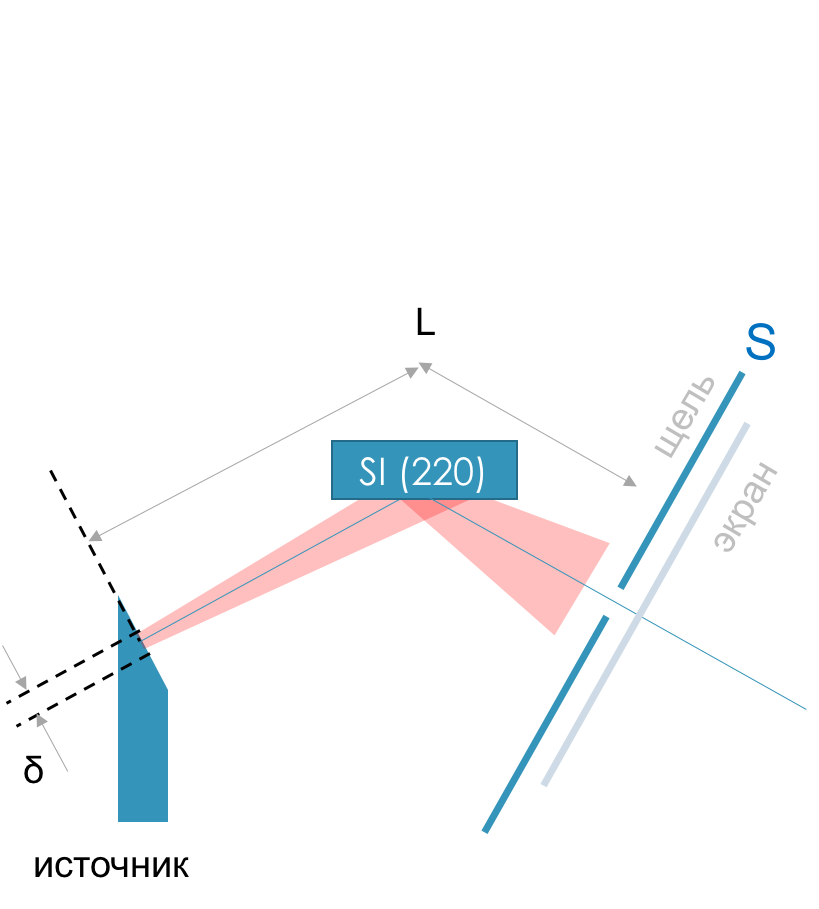
\includegraphics[width=0.45\textwidth]{images/single_crystal_schem.png}\label{ris:single_crystal_schem_lamtet_a}}
  \hfill
  \subfloat[Спектрально угловое распределение. Положение щелевых устройств обозначено синей линией вблизи $\pm 20$ угл.сек.
   ]{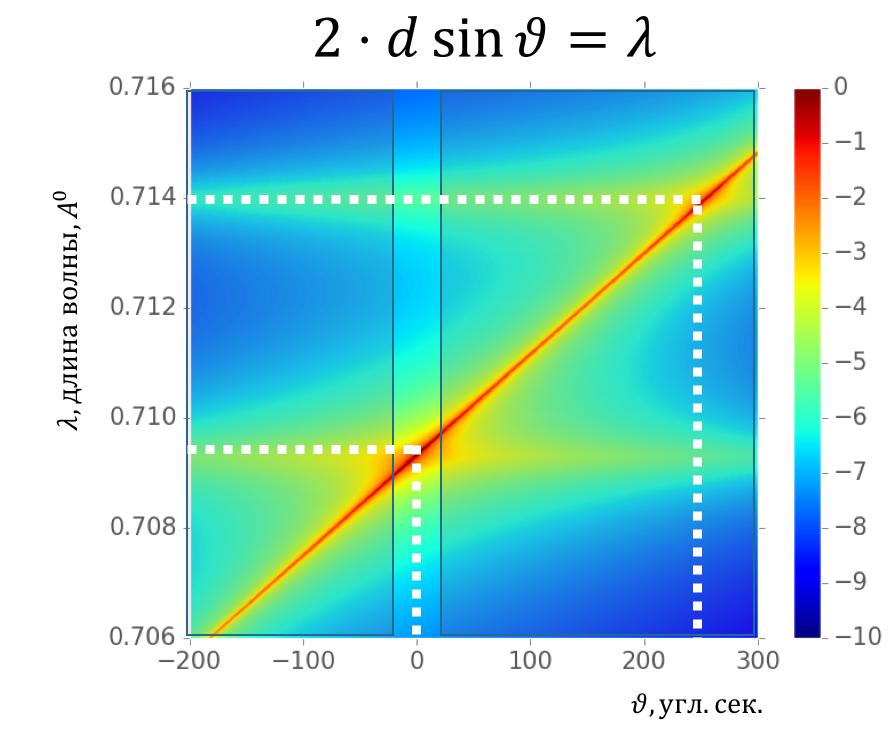
\includegraphics[width=0.45\textwidth]{images/single_crystal_schem_lamtet.png}}

  \caption{Спектрально угловое распределение после отражения расходящегося, полихромотического пучка от кристалла Si(220)}
  \label{ris:single_crystal_schem_lamtet}
\end{figure}

На рисунке \ref{ris:single_crystal_schem_lamtet}, по своей сути, изображен принцип работы монохроматора,
когда после взаимодействия с кристаллом, разные длины волн отражаются под разными углами в
соответсвии с законом Брегга.

Кривая отражения в однокристальном эксперименте (рисунок \ref{ris:single_crystal_schem_lamtet_a}), в котором сканирование осуществляется
 с помощью детектора жестко связанного с щелевым устройством линейного размера S, находящегося на расстоянии $L$ от источника, задается следующим образом

\begin{equation} \label{eq:p_single_crystal}
  P_{single}(\theta) = \sum_{\lambda = -\infty}^{\infty}g_{\lambda}(\lambda) \cdot \sum_{\vartheta = \vartheta_{s1}}^{\vartheta_{s2}}
  g_{\vartheta}(\vartheta) P_M(\vartheta - \frac{\lambda - \lambda_1}{\lambda_1}\tan(\theta_B))
 \end{equation}

где $\vartheta$ - угол падения излучения на кристалл, в случае не расходящегося пучка $\vartheta = 0$, в
случае, например, синхротронного источника $\vartheta \in (-6^o; 6^o) $; $g_{\lambda}(\lambda)$
- спектральная плотность распределения пучка (\ref{eq:source_spectral}); $g_{\vartheta}(\vartheta)$ - угловая плотность
распределения пучка (\ref{eq:source_angle}); $P_M$ - коэффициент отражения от неподвижного кристалла, далее мы будем его называть монохроматором,
слагаемое $\frac{\lambda - \lambda_1}{\lambda_1}\tan(\theta_B)$ -
возникает из условия Брегга и говорит о том, что разные длины волн отражаются под разными углами.
 Суммирование проводится сначала вдоль угловой апертуры детектора, которая задается размером
 щелевого коллиматора перед ним, а пределы определяются исходя из ее углового положения $\theta$ относительно
 оптической оси (зеркально отраженного луча) $\vartheta_{s1} = \theta - \frac{S}{2L}$, $\vartheta_{s2} = \theta + \frac{S}{2L}$,
 $S $ - линейный размер щелевого устройства, $L$ - расстояние от источника до щели.



На рисунке \ref{ris:zero_exp} приведен результат сканирования расходящегося пучка от рентгеновской
трубки после отражения от неподвижного кристалла кремния Si(220) для разных размеров щелевого коллиматора
в сравнении с расчетными.

   \subsubsection{Дифракция на щели}
      Cowley1979ru на странице 47
